% !TeX encoding = UTF-8
% !TeX root = V29_AFM.tex
% !TeX spellcheck = de_DE_frami

\section{Versuchsaufbau}
In unserem Versuchsaufbau wird ein AFM der Firma \emph{Nanosurf} mit der Typbezeichnung \emph{easyScan E-AFM} verwendet. Dieses befindet sich auf einem magnetischen Stabilisator, welcher für eine möglichst ebene Arbeitsoberfläche frei von störenden Vibrationen sorgt.\\
Der schematische Aufbau des AFM ist in Abbildung \ref{fig:AFM_schematic} zu sehen.
\begin{figure}[p]
	\centering
	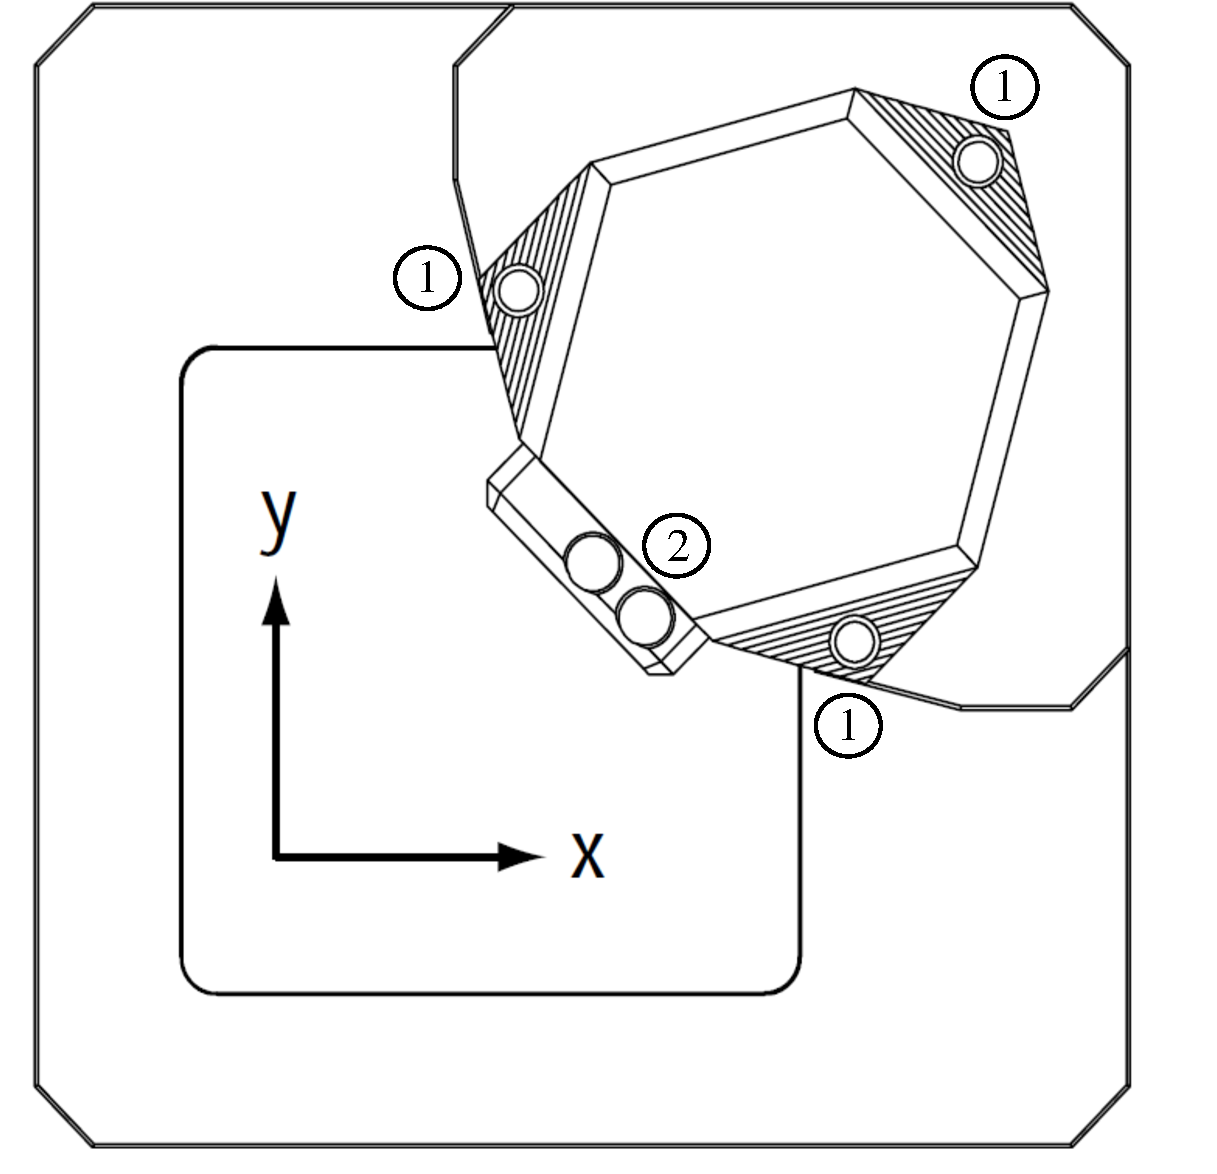
\includegraphics[width=\textwidth]{Nanosurf_e-afm_schematic.pdf}
	\caption[Schematischer Aufbau des \emph{Nanosurf} E-AFM]{Schematischer Aufbau des \emph{Nanosurf} E-AFM: An der Unterseite wird der Cantilever mittels einer Pinzette in eine Halterung angebracht. Die Grobeinstellung der Höhe geschieht mittels dreier Stellschrauben \ding{192}, welche sich triangular am Gerät befinden. Durch die zwei optischen Linsen \ding{193} lässt sich der Cantilever jeweils von oben und von der Seite aus betrachten. So kann die Funktionsfähigkeit des Cantilevers und der Abstand zur Probe festgestellt werden.}
	\label{fig:AFM_schematic}
\end{figure}
Das E-AFM wird bei unserem Versuch immer im contact mode mit \emph{constant force} betrieben, d.h. wir erhalten bei der Messung des Probenprofils entlang einer Linie das elektrische Signal des Rückkopplungskreises. Diese kann in eine tatsächliche Höhe $z$ umgerechnet werden.\\
Mit der Grobeinstellung wird der E-AFM mittels einer kleinen Wasserwaage waagrecht ausgerichtet, sodass Verzerrungen der Messungen durch die Gravitation in erster Näherung ausgeschlossen werden können.\\
Mit der beiliegenden Software des E-AFMs kann die Feineinstellung der Höhe des Cantilevers vorgenommen werden. Dazu kann man manuell die Höhe des Cantilevers einstellen, zur Kontrolle sollte man immer einen Blick auf die seitliche Ansicht des Cantilevers haben. Für die Messung fährt man den Cantilever so nah an die Probenoberfläche ran, sodass der Schatten des Cantilevers auf der Probe sichtbar wird. Anschließend lässt man das Programm automatisch den Cantilever an die Probe heranfahren, bis sie sich im Kontakt befinden.\\
Vor der eigentlichen Messung lassen sich noch die Winkelneigung in $x$- und $y$-Richtung (xSlope bzw. ySlope), den Messbereich (xRange, yRange), die Drehung sowie Offsets der Koordinatenachsen einstellen.\\
Für den auszumessenden Bereich der Probe, welches in ein Raster eingeteilt ist, lässt sich neben dem Bereich sowohl die Anzahl der Samples pro Linie als auch die dafür vorgesehene Zeitspanne einstellen. Eine hohe Anzahl von Samples ist zwar wünschenswert, wird aber durch die Geometrie der Spitze am Cantilever begrenzt. Für die Zeit pro Linie gilt pauschal, dass eine längere Zeit für meist bessere Messergebnisse sorgt, u.a. weil der sogenannte \emph{overshoot} nach einer abrupten Höhenänderung im Profil gegenüber dem umgebenden Plateaus kürzer ausfällt. Jedoch kann die Probe bei zu langer Kontaktdauer beschädigt werden.\\
Jede Linie in diesem Raster wird doppelt ausgemessen (ForwardScan und BackwardScan). Daraus kann die Kraft zwischen Spitze und Probe ermittelt werden.\\
Im Ansichtsfenster (ScanPanel) lassen sich zudem verschiedene Fenster einblenden, welche bspw. das Höhenprofil der gescannten Linie oder die Oberansicht des abgerasterten Ausschnitts anzeigen.
\section{Versuchsdurchführung und -auswertung} 
\subsection{Ermittlung der optimalen Parameter für die Messungen}
Im Idealfall liegt die abzumessende ebene Probe in der $x$-$y$-Ebene des AFMs. Eine vorhandene Neigung der Probenebene zur idealen Messebene lässt sich durch die Eingabe geeigneter Winkel in die Felder \emph{X-Slope} und \emph{Y-Slope} kompensieren. Die Messung der noch nicht ausgerichteten Ebene - bei unserem Versuch wurde eine glatte Siliziumoberfläche %not sure about that
als Referenz genommen - ist in Abbildung \ref{fig:tilt} zu sehen.
\begin{figure}[h]
	\centering
	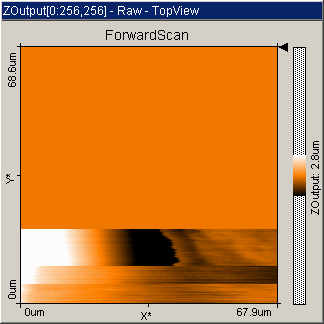
\includegraphics[width=0.5\textwidth]{tilt_tip0.png}
	\caption{Nicht ausgerichtete Probenoberfläche.}
	\label{fig:tilt}
\end{figure}
Mit der Einstellung $X$-Slope=+1,5\degree konnte dieser Tilt beseitigt werden.

Im Folgenden gilt es, die idealen Einstellungen für den \emph{P-Gain} und \emph{I-Gain} empirisch zu ermitteln. Über den Rückkopplungskreis des AFM erhalten wir eine Abweichung, welche entweder proportional (P) oder integral (I) verstärkt als Signal an den $z$-Pi\"{e}zo zurückgegeben wird, welcher die Höhe des Cantilevers steuert.\\
Ein zu niedriger Wert bewirkt eine zu langsame Reaktion des Systems auf Änderungen in der Topologie der Probe, während ein zu hoher Wert das System sehr empfindlich gegen Oszillationen und Störungen werden lässt.

In der Abbildung \ref{fig:gain} ist eine Messung an einem Kalibrationsgitter für verschiedene Wertepaare (P,I) der Gains zu sehen, anhand dessen wir die optimalen Werte abschätzen.
\begin{figure}[h]
	\centering
	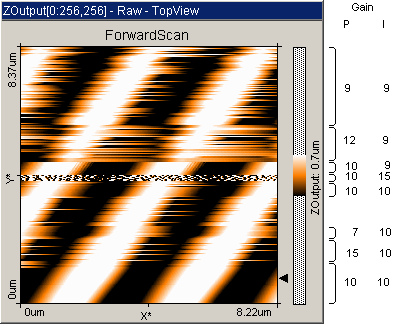
\includegraphics[width=0.7\textwidth]{lattice_tip2_1b_legend.png}
	\caption[Bestimmung des P- und I-Gains]{Messung an einem Kalibrationsgitter für verschiedene P- und I-Gains.}
\label{fig:gain}
\end{figure}
Anhand dieser Messungen erhalten wir als ideale Werte P=10 und I=10. Dies entspricht auch der Empfehlung im Handbuch des verwendeten AFMs.
\subsection{Kalibration und Charakterisierung der Spitze}
Zuerst wurde eine glatte Silizium-Oberfläche mit dem AFM abgerastert. Das dabei entstandene Bild ist in Abbildung \ref{fig:Si_smooth01} zu sehen.
\begin{figure}[h]
	\centering
	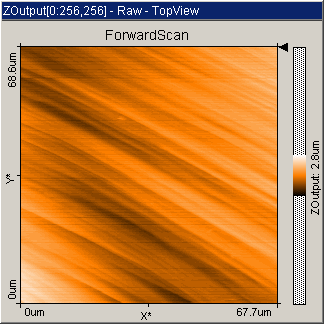
\includegraphics[scale=0.5]{Si_smooth01.png}
	\caption{Messung einer glatten Silizium-Oberfläche.}
	\label{fig:Si_smooth01}
\end{figure}
Es ist festzustellen, dass die Oberfläche nicht ideal glatt ist, sondern eine beinahe periodische Struktur aufweist. Zudem befindet sich ein Tal im abgerasterten Bereich. Dieses Tal entsteht durch die Verwendung von Rohrscannern zur Bewegung des Cantilevers.

Als nächstes erfolgte eine Messung an einem Kalibrationsgitter aus Silizium. Die Abbildung \ref{fig:Si_grating} zeigt den schematischen Aufbau des Gitters.
\begin{figure}[H]
	\centering
	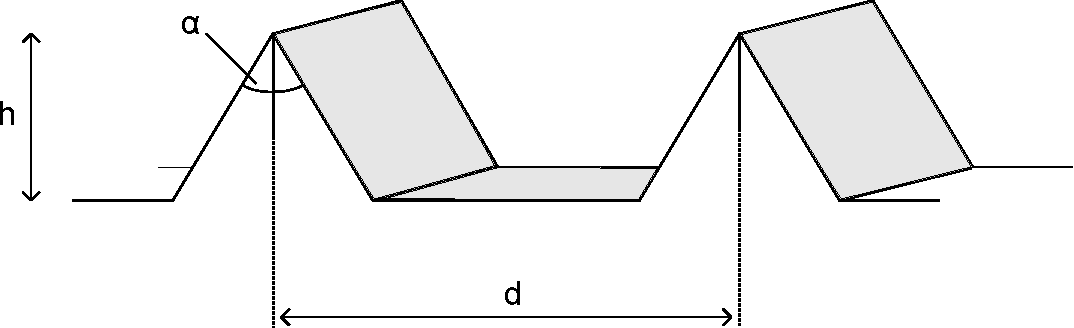
\includegraphics[scale=0.7]{Si_grating.pdf}
	\caption[Schematischer Aufbau des Silizium-Kalibrationsgitters]{Schematischer Aufbau des Silizium-Kalibrationsgitters. Laut der Spezifikation beträgt der Abstand $d$ von zwei Kanten 3\micro\metre, die Höhe $h$ einer Kante 1,8\micro\metre{} und der Winkel $\alpha$ an der oberen Kante 70\degree.}
	\label{fig:Si_grating}
\end{figure}
Die ersten Messungen am Gitter sind in Abbildung \ref{fig:Lattice1} zu sehen. Bei näherer Betrachtung (vgl. Abbildung \ref{fig:Lattice2}) ist zu erkennen, dass die ursprünglich triangulare Form der Kanten nicht mehr wiedergegeben wird. Es wird ein Defekt der Spitze am Cantilever vermutet, weswegen dieses anschließend ausgetauscht wurde.
\begin{figure}[H]
	\centering
\begin{minipage}{0.45\textwidth}
\centering
		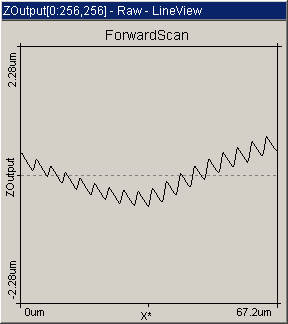
\includegraphics[scale=0.5]{lattice02.png}
		\caption*{a) $Z$-Profil}
	\end{minipage}
	\hfill
\begin{minipage}{0.45\textwidth}
\centering
		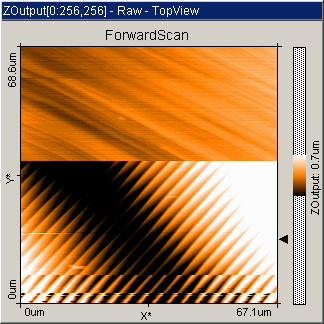
\includegraphics[scale=0.5]{lattice03.png}
		\caption*{b) Oberansicht}
	\end{minipage}
	\caption[Erste Messungen am Kalibrationsgitter]{Erste Messungen am Kalibrationsgitter:\\ $X$-Range 60\micro\metre,  Variation der Scan-Zeit von 0,4$\rightarrow$ 1 $\rightarrow$ 2\second\per line.}
	\label{fig:Lattice1}
\end{figure}

\begin{figure}[H]
\centering
\begin{minipage}{0.45\textwidth}
\centering
		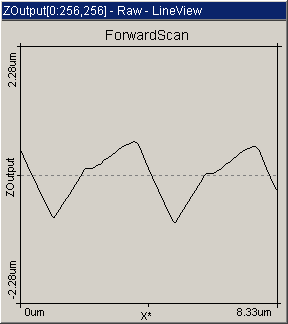
\includegraphics[scale=0.5]{lattice05.png}
		\caption*{a) $Z$-Profil}
	\end{minipage}
	\hfill
\begin{minipage}{0.45\textwidth}
\centering
		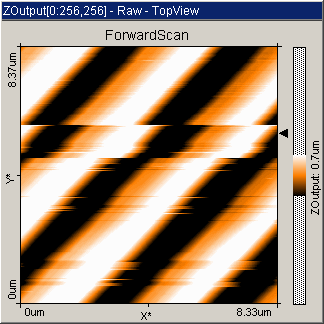
\includegraphics[scale=0.5]{lattice04.png}
		\caption*{b) Oberansicht}
	\end{minipage}
	\caption[Messung mit $X$-Range=8\micro\metre]{Messung mit $X$-Range=8\micro\metre. Die Messung wurde durch Schalleinwirkung seitens der Probanden erheblich beeinflusst.}
	\label{fig:Lattice2}
\end{figure}

Mit dem neuen Cantilever wurde anschließend eine weitere Messung an einer glatten Silizium-Oberfläche vorgenommen. Dabei wurde - unbeabsichtigt - ein Staubpartikel mit erfasst, dies ist deutlich in der Abbildung \ref{fig:Si_particle} zu sehen. Die Höhe des betrachteten Partikels ist $(0,17 \pm 0,04)\micro\metre$, für die maximale Breite wurde $(0.99 \pm 0,11)\micro\metre$ ermittelt.
\begin{figure}[H]
\centering
	\begin{minipage}{0.45\textwidth}
	\centering
		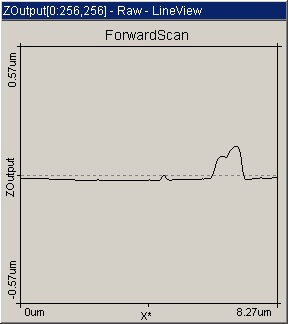
\includegraphics[scale=0.5]{Si_tip2_particle_a.png}
		\caption*{a) $Z$-Profil}
	\end{minipage}
	\hfill
	\begin{minipage}{0.45\textwidth}
	\centering
		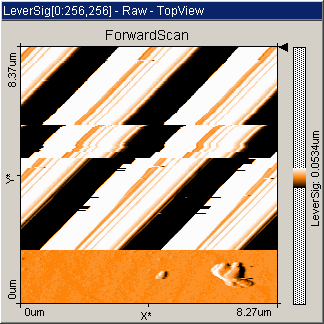
\includegraphics[scale=0.5]{Si_tip2_particle_c_contrast.png}
	\caption*{b) Oberansicht}
	\end{minipage}
	\caption[Messung mit Staubpartikel]{Messung mit neuen Cantilever an einer glatten Silizium-Oberfläche und versehentlicher Erfassung eines Staubpartikels.}
	\label{fig:Si_particle}
\end{figure}

Daraufhin wurde wiederum das Kalibrationsgitter ausgemessen, die entsprechenden Bilder befinden sich in Abbildung \ref{fig:Lattice3}.
\begin{figure}[h]
\centering
	\begin{minipage}{0.45\textwidth}
	\centering
		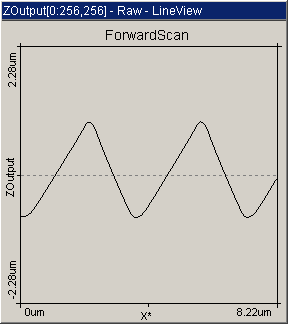
\includegraphics[scale=0.5]{lattice_tip2_1a.png}
		\caption*{a) Z-Profil}
	\end{minipage}
	\hfill
	\begin{minipage}{0.45\textwidth}
	\centering
		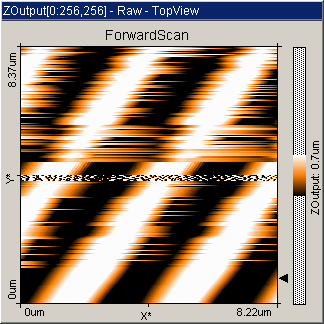
\includegraphics[scale=0.5]{lattice_tip2_1b.png}
		\caption*{b) Oberansicht}
	\end{minipage}
	\caption[Zweite Messung am Kalibrationsgitter]{Zweite Messung am Kalibrationsgitter. Die Messung erfolgte nur über die unteren 15\% des Bildes.}
	\label{fig:Lattice3}
\end{figure}
Wir erhalten
\begin{align*}
\text{Höhe: }h&=(1,43\pm 0,02)\micro\metre\\
\text{Abstand zwischen zwei Kanten: }d&=(3,84 \pm 0,02)\micro\metre\\
\text{Winkel der Kante: }\alpha&=(84,1\pm 0,2)\degree
\end{align*}
Die Ursache für die vom Datenblatt abweichenden Maße ist die Tatsache, dass die Erfassung des Höhenprofils nicht senkrecht zu den Kanten stattfand, sondern vielmehr schräg über das Gitter. Dies wurde für die weiteren Messungen korrigiert.
\subsection{Messung verschiedener Proben}
\subsubsection{CD}
Ein weiterer Teil der Aufgabenstellung ist die Messung der Oberflächenstruktur einer mit Daten beschriebenen CD.\\
Die Daten werden bei der Herstellung auf die Schicht aus Polycarbonat (PC) in Form von Vertiefungen, den sogenannten \emph{pits}, in eine spiralförmige Spur gebrannt, welche sich von der Mitte der CD nach außen zieht. Der Abstand zwischen zwei Spuren beträgt 1,5\micro\metre. Sie haben typischerweise eine Tiefe von etwa 100\nano\metre und eine Länge von $850\nano\metre$ bis $3,5\micro\metre$ (gemäß \cite{lit:wiki_cd}).\\
Für die Messung wird mittels eines Skalpells die reflektierende Aluminiumschicht, welche das Negativ der beschriebenen PC-Schicht darstellt aus der CD ausgeschnitten.\\
Eine Messung ist in Abbildung \ref{fig:CD} zu sehen.
\begin{figure}[h]
\centering
	\begin{minipage}{0.45\textwidth}
	\centering
		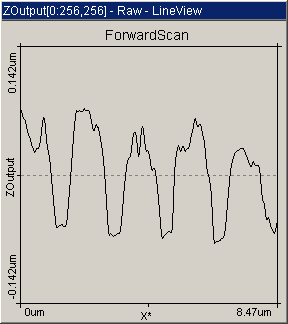
\includegraphics[scale=0.5]{cd_1,0s_a.png}
		\caption*{a) $Z$-Profil}
	\end{minipage}
	\hfill
	\begin{minipage}{0.45\textwidth}
	\centering
		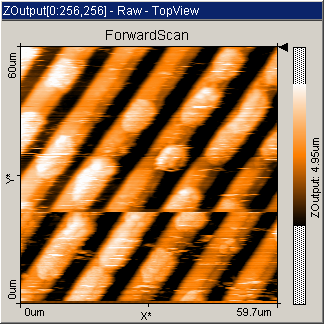
\includegraphics[scale=0.5]{cd_1,0s_b_best.png}
		\caption*{b) Oberansicht}
	\end{minipage}
	\caption{Aufnahme einer CD.}
	\label{fig:CD}
\end{figure}
Aus den Abbildungen ist zu entnehmen:
\begin{align*}
\text{Abstand zwischen zwei Spuren: }& (1,9\pm0,5)\micro\metre\\
\text{Tiefe der pits (abgeschätzt): }& (0,2\pm0,1)\micro\metre\\
\text{Länge des kürzesten pits: }& 8\micro\metre 
\end{align*}
Der Abstand der Spuren und die Tiefe der pits entsprechen weitgehend den üblichen Ausmaßen, die Länge der pits divergiert allerdings. Das Ausmessen wird erheblich erschwert durch einen schlecht gewählten farblichen Kontrast, sowie durch die Artefakte. Diese enthalten u.a. overshoots, und Oszillationen von außen. Es ist außerdem nicht ohne weiteres erkennbar, ob es sich um eine gepresste oder gebrannte CD handelt.
\subsubsection{Biologische Probe}
Eine weitere Aufgabenstellung ist, eine biologische Probe mit dem AFM auszumessen. Hierzu wurde ein Haupthaar einem der Probanden entnommen und auf einem Deckglas präpariert. Die Abbildung \ref{fig:hair} enthält die dabei erstellten Aufnahmen.
\begin{figure}[h]
\centering
	\begin{minipage}{0.45\textwidth}
	\centering
		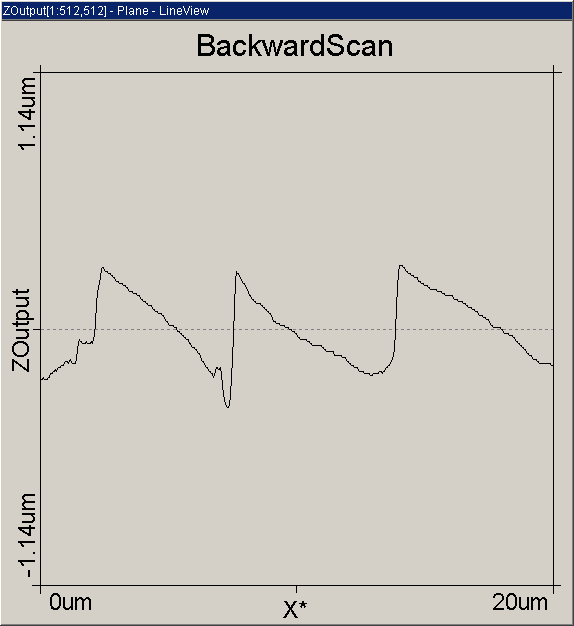
\includegraphics[scale=0.3]{hair_1,5s_512_a.png}
		\caption*{a) $Z$-Profil}
	\end{minipage}
	\hfill
	\begin{minipage}{0.45\textwidth}
	\centering
		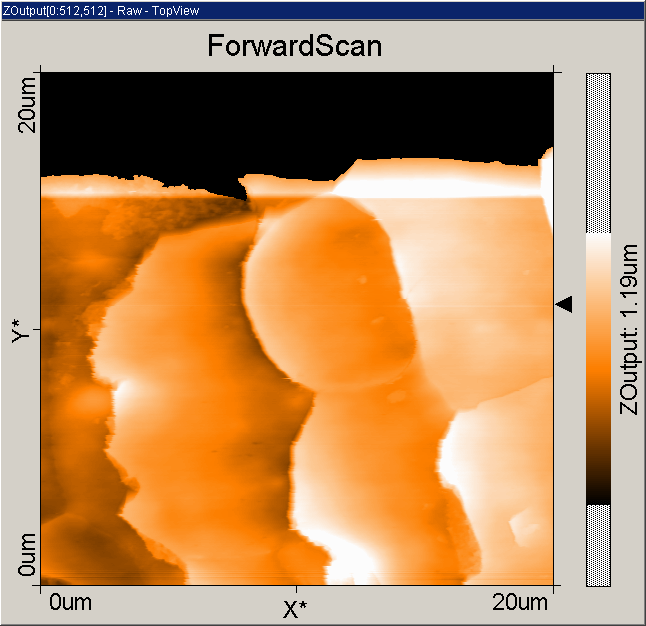
\includegraphics[scale=0.3]{hair_1,5s_512_b.png}
		\caption*{b) Oberansicht}
	\end{minipage}
	\caption{Messung am Haar}
	\label{fig:hair}
\end{figure}
Deutlich ist die Cuticula, die äußere Schuppenschicht zu erkennen. Das aufgenommene Bild weist lediglich die üblichen overshoots nach scharfen Übergängen auf. Außerdem kommt es zu unscharfen Abgrenzungen am Rand der Haarprobe, da die Spitze an der Probe abrutscht.
\subsection{Kraft-Distanz-Kurven}
\subsubsection{Messung auf einer glatten Silizium-Probe}
Es wurde wiederum eine glatte Silizium-Probe ausgemessen. Dieses Mal ließen wir uns in einem Spektrograph die gemessene Kraft - genauer die Verbiegung des Cantilevers - gegen den Abstand der Spitze zur Probe auftragen. Diese werden entlang einer Linie mit einer vorgegebenen Anzahl an samples aufgenommen.\\
Dabei wird die Kraft im \emph{ForwardSpec}, d.h. die Spitze wird auf die Probe aufgesetzt, und im \emph{BackwardSpec}, hier wird der Abstand Spitze-Probe wieder vergrößert, aufgezeichnet.\\
Im Verlauf dieser Messung hauchte ein Proband auf die Silizium-Probe, sodass ein (zusätzlicher) dünner Wasserfilm auf der Probe entstand. Diese beeinflussen die Kraft-Distanz-Kurve (KDK) durch die dadurch entstandene zusätzliche Adhäsion.

Die entsprechenden Kraft-Distanz-Kurven befinden sich in Abbildung \ref{fig:Si_force-distance}.
\begin{figure}[h]
\centering
	\begin{minipage}{0.32\textwidth}
	\centering
		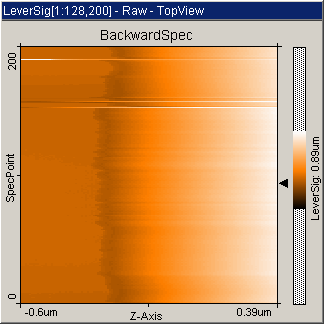
\includegraphics[scale=0.5]{Si_F(z)_1s_b.png}
		\caption*{a) $F(z)$ entlang der Linie}
	\end{minipage}
	\hfill
	\begin{minipage}{0.28\textwidth}
	\centering
		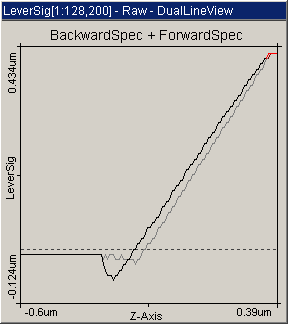
\includegraphics[scale=0.5]{Si_F(z)_1s_bare_a_scaled.png}
		\caption*{b) KDK ohne Wasserfilm}
	\end{minipage}
	\hfill
	\begin{minipage}{0.28\textwidth}
	\centering
		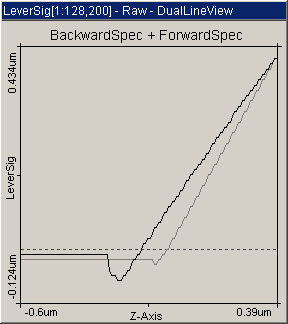
\includegraphics[scale=0.5]{Si_F(z)_1s_breath_a_scaled.png}
		\caption*{c) KDK mit Wasserfilm}
	\end{minipage}
	\caption[Kraft-Distanz-Kurven auf glattem Silizium]{Kraft-Distanz-Kurven (KDK) auf glattem Silizium, die schwarze Kurve ist der BackwardSpec und die graue Kurve der ForwardSpec.\\ a) Gemessener Kraftverlauf entlang der Linie. Das obere Fünftel zeigt die Messung mit Wasserfilm.\\ b) KDK ohne Wasserfilm\\ c) KDK mit Wasserfilm.}
	\label{fig:Si_force-distance}
\end{figure}
Die Kraft-Distanz-Kurven sind über das gewählte Messintervall weitgehend ähnlich. Die Unterschiede beruhen auf lokale Unreinheiten, wie dünne Lagen von Wassertröpfchen (da die Messung in Luft stattfand und somit durch die Luftfeuchtigkeit Wasser kondensiert) sowie mögliche Unebenheiten der Probe selbst.\\ 
Bei der Vorwärtsbewegung der Spitze gegen die Probe ist bei nicht-Kontakt keine Kraftänderung festzustellen. Bei sehr geringem Abstand kommt die Van-der-Waals-Kraft zum Tragen, welche anziehend wirkt. Ab dem Punkt, an dem die Spitze Kontakt zur Probe hat, ist die Kraft weitgehend linear zum Abstand. Dies ist der Hooksche Bereich des Elastizitätsmoduls des Cantilevers.\\
Bewegen wir die Spitze wieder weg von der Probe, so ist der Verlauf weitgehend identisch zur Annäherung, er unterscheidet sich um einen geringen Offset. Dies ist der Hysterese des Cantilevers verschuldet.\\
Befindet sich nun ein Wasserfilm auf der Probe, zu sehen in Abbildung \ref{fig:Si_force-distance}c) und abgeschwächt auch schon in \ref{fig:Si_force-distance}b), so bewirkt die durch den Film verursachte Adhäsion eine weitere Anziehung der Probe. Ab einem gewissen Punkt wird mit dem weiterem Entfernen der Spitze von der Probe auch diese Kraft überwunden, und der Cantilever springt in die Ruhelage zurück. Dies ist der \emph{snap-back}.\\
Die ForwardSpec-Kurven der Messung ohne und mit Wasserfilm müssten auf derselben Position liegen, vermutlich ist der Offset dem Hauchen auf die Apparatur verschuldet, sodass sich auch auf dem Cantilever Flüssigkeit angesammelt haben könnte.
Berücksichtigen wir diesen Offset, so ist der Unterschied der BackwardSpec-Kurven mit und ohne Wasserfilm wesentlich verständlicher; die stärkere Adhäsion bewirkt eine anziehende Kraft über einen größeren Abstand der Spitze zur Probe.
Die kleinen Oszillationen in den Kraft-Distanz-Kurven sind dem Bitrauschen zuzuordnen, welche durch die Diskretisierung des Messbereich in samples entstehen.
\subsubsection{Messung auf einer mit SBR versetzten Silizium-Probe}
Analog zum vorherigem Schritt wurde eine Silizium-Probe ausgemessen, welche mit \emph{Styrol-Butadien-Kautschuk} (SBR) in Form von Tropfen versetzt wurde. Beim SBR handelt es sich um ein synthetisches Gummi, welches bei Raumbedingungen ein viskoelastisches Verhalten aufweist.
Das abgetastete Intervall verläuft über drei dieser ``Flecken'' und ist in Abbildung \ref{fig:cow_line} veranschaulicht.
\begin{figure}[h]
	\centering
	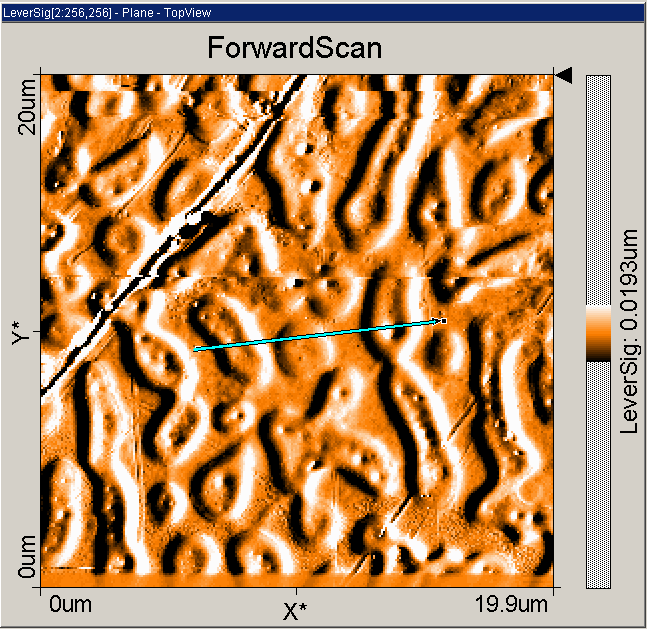
\includegraphics[scale=0.5]{cow_c_0,7s_line.png}
	\caption[Messung einer SBR-Silizium-Probe]{Messung einer SBR-Silizium-Probe: Das abgerasterte Intervall ist in türkis eingezeichnet.}
	\label{fig:cow_line}
\end{figure}
Wird das Rückkopplungssignal des Cantilevers in tatsächliche Höhe umgerechnet, so ergibt sich das Bild in Abbildung \ref{fig:cow_z}.
\begin{figure}[h]
	\centering
	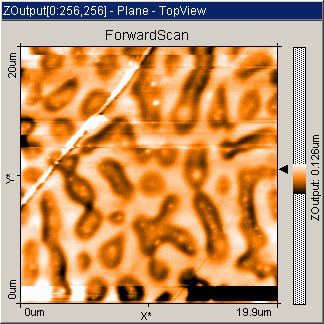
\includegraphics[scale=0.7]{cow_scan_0,7s_b.png}
	\caption{Aufnahme der SBR-Probe mit Höhenprofil.}
	\label{fig:cow_z}
\end{figure}
Betrachten wir nun die über die in \ref{fig:cow_line} zu sehenden Linie aufgenommenen Kraft-Distanz-Kurven, so erhalten wir im Spektrographen die Abbildung \ref{fig:cow_spec}a). Es ist zu erkennen, dass bei den Übergang von einem Plateau zu einem anderen die Kraft-Distanz-Kurve verschoben wird zu einer geringeren Abstand der Spitze zur Probe. Die KDK für einem tieferen bzw. höheren Plateau finden sich in Abbildung \ref{fig:cow_spec}b) bzw. \ref{fig:cow_spec}c).
\begin{figure}[H]
\centering
	\begin{minipage}{0.32\textwidth}
	\centering
		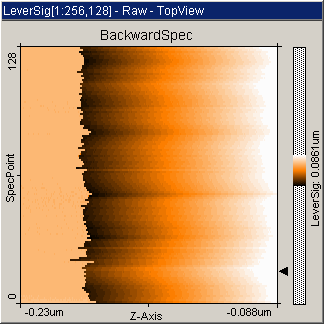
\includegraphics[scale=0.5]{cow_spec5_1s_b.png}
		\caption*{a) $F(z)$ entlang der Linie}	
	\end{minipage}
	\hfill
		\begin{minipage}{0.28\textwidth}
		\centering
		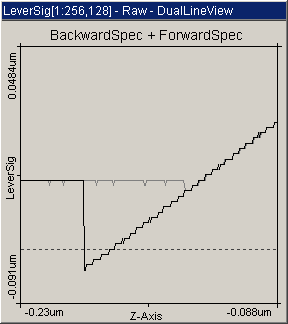
\includegraphics[scale=0.5]{cow_spec5_1s_a_dark.png}
		\caption*{\!b) KDK an dunklem Fleck\!\!}	
	\end{minipage}
	\hfill
	\begin{minipage}{0.28\textwidth}
	\centering
		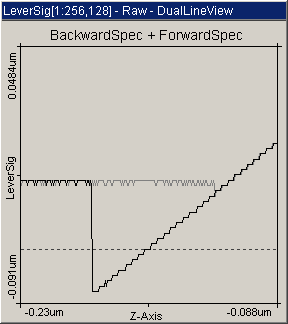
\includegraphics[scale=0.5]{cow_spec5_1s_a_bright.png}
		\caption*{c) KDK an hellem Fleck}	
	\end{minipage}
	\caption[Kraft-Distanz-Kurve der SBR-Probe]{KDK der SBR-Probe. \glqq Dunkle Flecken\grqq{} entsprechen tiefen Plateaus, \glqq helle Flecken\grqq{} höheren Plateaus.}
	\label{fig:cow_spec}
\end{figure}
Die Kraft-Distanz-Kurven entsprechend vom Verlauf weitgehend der auf glatten Silizium. Die KDK von tiefen und höheren Ebene sind ein wenig verschoben, zudem ist die anziehende Kraft bei der Messung der höheren Ebene etwas ausgeprägter.
\section{Fehlerdiskussion}
Die Messungen am AFM sind sehr anfällig gegen äußere Schwingungen, die nicht allesamt vom Stabilisator abgefangen werden können. Dazu zählen u.a. kurze Stöße am Tisch, Schwingungen von Geräten im Versuchsraum, aber hauptsächlich akustischer Schall durch sprechende Versuchsteilnehmer.\\
Es konnte nicht sichergestellt werden, dass die Spitze des Cantilevers im Laufe der weiteren Messungen weiterhin intakt geblieben ist.